%%
% Είδος: διπλωματική στα αγγλικά
\documentclass{uthece-thesis} 

% Πακέτα και ορισμοί που τυχόν χρειάζονται, ανάλογα με το κείμενο της διπλωματικής
\usepackage{algorithm}
\usepackage{algorithmic}

\usepackage[hyphens]{url}
\usepackage{multicol}
\usepackage{multirow}
\usepackage[table]{xcolor}
\usepackage{caption} 
\captionsetup[table]{skip=10pt}
\usepackage{tikz}
\usepackage{datetime}
\usepackage{ifthen}
\usepackage{hyperref} % Για ενεργά URLs
\usepackage{siunitx}

%%%%%%
% VASILEIOS DIMITRIOU
%αριθμός γενικού μητρώου: Μ011723007
%αριθμός μητρώου: 00578


% Πρόσθετοι ορισμοί, ανάλογα με το κείμενο της διπλωματικής
% typeset source code
\newcommand{\src}[1]{{\tt#1}}

% typeset a backslash
\newcommand{\bkslash}{\symbol{92}}

% Κύρια γλώσσα της διπλωματικής
% μην την τροποποιείτε
\ifgrthesisoption 
    \setlanguage{greek}
\else
    \setlanguage{american} 
\fi


%%%%%%%%%%%%%%%%%%%%%%%%%%%%%%%%%%%%%%%%%%%%%%%%%%%%%
%% THESIS INFO / ΠΛΗΡΟΦΟΡΙΕΣ ΔΙΠΛΩΜΑΤΙΚΗΣ
%%
% Τίτλος Διπλωματικής Εργασίας στα ελληνικά
	\title{Διερεύνηση Σχεδίασης Συστημάτων Ανάλυσης Δονήσεων Μηχανών}
% Τίτλος Διπλωματικής Εργασίας στα αγγλικά
	\titleEng{Investigation of Machine Vibration Analysis System Design}
% Ονοματεπώνυμο φοιτητή στα ελληνικά
	\edef\authorname{Βασίλειος Δημητρίου}
	\edef\secauthorname{}
% Ονοματεπώνυμο φοιτητή στα αγγλικά 
	\edef\authornameEng{Vasileios Dimitriou}
	\edef\secauthornameEng{}
% Ονοματεπώνυμο Επιβλέποντα Καθηγητή στα ελληνικά
	\supervisor{Καρακωνσταντής Γεώργιος}
% Ονοματεπώνυμο Επιβλέποντα Καθηγητή στα αγγλικά
	\supervisorEng{Karakonstantis Georgios}
% Φύλλο επιβλέποντα στα ελληνικά 
% Μην το τροποποιείτε για διπλωματική στα αγγλικά
	\edef\supervisorMaleFemale{Επιβλέπων/πουσα}
% Στοιχεία επιτροπής στα αγγλικά
    \edef\supervisortitle{Rank/position of Supervisor}
    \edef\supervisoraffiliation{Department of Electrical and Computer Engineering, University of Thessaly}
    \edef\memberonename{Name Surname of Member 1}
    \edef\memberonetitle{Rank/position of Member 1}
    \edef\memberoneaffiation{Department/Institution of Member 1}
    \edef\membertwoname{Name Surname of Member 2}
    \edef\membertwotitle{Rank/position of Member 2}
    \edef\membertwoaffiation{Department/Institution of Member 2}    
% Ημερομηνία υποβολής διπλωματικής
    \newdate{docdate}{04}{02}{2022}
% Ημερομηνία έγκρισης διπλωματικής
    \newdate{docapprovedate}{24}{02}{2022}
% format ημερομηνίας - μην το τροποποιείτε
    \newdateformat{mydate}{\THEDAY-\THEMONTH-\THEYEAR} \mydate
% Τόπος και έτος διπλωματικής στα ελληνικά
	\edef\thesisPlaceDate{Μήνας \getdateyear{docdate}}
% Τόπος και έτος διπλωματικής στα αγγλικά
	\edef\thesisPlaceDateEng{Month \getdateyear{docdate}}
%


%%%%%%%%%%%%%%%%%%%%%%%%%%%%%%%%%%%%%%%%%%%%%%%%%%%%


\begin{document}

\frontmatter
\maketitle


%%%%%%%%%%%%%%%%%%%%%%%%%%%%%%%%%%%%%%%%%%%%%%%%%%%%%
%% OPTIONAL MATERIAL / ΠΡΟΑΙΡΕΤΙΚΕΣ ΕΝΟΤΗΤΕΣ
%%
% Κατάλογος Σχημάτων προαιρετικά
	\listoffigures % σε σχόλια για μη εμφάνιση
% Κατάλογος Πινάκων προαιρετικά
%	\listoftables % σε σχόλια για μη εμφάνιση
% Συντομογραφίες - Αρκτικόλεξα - Ακρωνύμια προαιρετικά
	% Συντομογραφίες - Αρκτικόλεξα - Ακρωνύμια

\newcommand{\abbrev}[2]{#1 \> #2\\ }
\begin{abbreviations}

\begin{tabbing}
%ta 'a' rythmizoun to platos ton dyo stilon
  aaaaaaaaaaaaaaaaa \= aaaaaaaaaaaaaaaaaaaaaa\kill
  \abbrev{βλπ}{βλέπε}
  \abbrev{κ.λπ.}{και λοιπά}
  \abbrev{κ.ο.κ}{και ούτω καθεξής}
  \abbrev{ΤΕΙ}{Τεχνολογικό Εκπαιδευτικό Ίδρυμα}
  \abbrev{BPF}{Band Pass Filter}
\end{tabbing}
\end{abbreviations} % σε σχόλια για μη εμφάνιση 
%
%%%%%%%%%%%%%%%%%%%%%%%%%%%%%%%%%%%%%%%%%%%%%%%%%%%%


\mainmatter
%%%%%%%%%%%%%%%%%%%%%%%%%%%%%%%%%%%%%%%%%%%%%%%%%%%%%
%% CHAPTERS / ΚΕΦΑΛΑΙΑ 
%%
    \chapter{Introduction}
\label{chap1}

Motivation and description
Εδώ αυτή κάνουμε μια γενική περιγραφή του χώρου εφαρμογής της διπλωματικής. Αναφέρουμε τα χαρακτηριστικά του χώρου και καταλήγουμε στα γενικότερα προβλήματα που αντιμετωπίζει ο χώρος. Η συζήτηση των προβλημάτων θα πρέπει να προϊδεάζει τον αναγνώστη για το τι θα προσπαθήσει να αντιμετωπίσει η διπλωματική, χωρίς ακόμα να αναφερόμαστε συγκεκριμένα στο αντικείμενο της διπλωματικής.
  


\section{Αντικείμενο της διπλωματικής}

Εδώ αναφερόμαστε συγκεκριμένα στο τί θα κάνει η διπλωματική. Αναφέρουμε λεπτομερώς α) τα προβλήματα που θα λύσει (και που ήδη έχουν περιγραφεί γενικά στην προηγούμενη ενότητα), και β) πώς σκοπεύει να τα λύσει. 
Είναι σημαντικό κάποιος που θα διαβάσει την ενότητα αυτή να καταλάβει σε σημαντικό βαθμό τον σκοπό της διπλωματικής σας και τις τεχνικές δυσκολίες της, χωρίς να είναι αναγκαίο να δει όλα τα άλλα κεφάλαια. Η ενότητα αυτή θέλει πολύ προσοχή και καλύτερα να τη γράψετε αφού έχετε γράψει όλα τα υπόλοιπα κεφάλαια.

\subsection{Συνεισφορά}
Εδώ παραθέτουμε αριθμητικά συγκεκριμένες ενέργειες/λύσεις/μεθοδολογίες που παρουσιάζει η διπλωματική και λύνουν τα προβλήματα που υποσχεθήκαμε στην προηγούμενη ενότητα ότι θα λύσει η διπλωματική. Συνήθως η υποενότητα αυτή έχει την παρακάτω μορφή:

Η συνεισφορά της διπλωματικής συνοψίζεται ως εξής:
\begin{enumerate}
\item Μελετήθηκαν συστήματα κ.λ.π.
\item Υλοποιήθηκαν τρεις αλγόριθμοι υπολογισμού κ.λ.π.
\item Αξιολογήθηκε η επίδοση των αλγορίθμων και βρέθηκε ότι κ.λ.π.
\item Ενσωματώθηκαν οι αλγόριθμοι σε πρότυπο σύστημα κ.λ.π.
\item ...
\end{enumerate}


\section{Οργάνωση του τόμου}

Εδώ περιγράφουμε τα κεφάλαια της διπλωματικής: μία πρόταση για το τί θα έχει  κάθε κεφάλαιο.Συνήθως η ενότητα αυτή έχει την παρακάτω μορφή (δεν θα σας πάρει πάνω από μία μεγάλη παράγραφο):

Εργασίες σχετικές με το αντικείμενο της διπλωματικής παρουσιάζονται στο Κεφάλαιο \ref{chap2}. Το Κεφάλαιο ... συζητά θέματα μοντελοποίησης. Στο Κεφάλαιο ... αναπτύσσουμε κ.λ.π. 

Για την τελική οργάνωση του κειμένου σας, συμβουλευθείτε τον επιβλέποντα της εργασίας.



    \chapter{Theoretical Background}
\label{chap2}
\section{Fundamentals of Bearing Fault Frequencies}
{
\subsection{Overview}
{
The most significant challenge that the authors had to deal with is that of the faulty cases detection. For this reason, fault and unfault models have been developed, and series of comparisons between the actual model generated by apparatus measurements and these two situational models are being executed. This development constitutes a real challenge since this is the main criterion that identifies the state of the motor.
}

\subsection{Unfault and Fault Models}
{
As previously mentioned, the authors make use of a model-based approach, which entails that the main concept is comparison-oriented. Specifically, there is the unfault model, which contains a high-amplitude peak at the shaft rotating frequency $F_{\omega}$. In addition to that, it can be noticed in Figure~\ref{fig:faultsunfaults} that some other patterns distinct themselves from the previously-mentioned unfault model. Regarding the unbalance model, it is obvious that the amplitude at the first tone is much greater. In the case of the misalignment model, it can be noticed that the tone at $2F_{\omega}$ has a much greater amplitude while the amplitude at the tone of the shaft speed $F_{\omega}$ remains at a high level. In the case of looseness, there are some more tones prevailing on the spectrum, among the tones related to the shaft speed. To top it all off, the most important vibration spectrum is that of the bearing failure (Refer to Figure~\ref{fig:faultTree}). Every bearing is characterized by four critical frequencies, given by its manufacturer, and these frequencies are associated with the four bearing components (inner and outer ring, balls, and cage):

\begin{itemize}
	\item BPFO (Ball Pass Frequency Outer) - outer race failure
	\item BPFI (Ball Pass Frequency Inner) - inner race failure
	\item BSF (Ball Spin Frequency) - rolling element failure
	\item FTF (Fundamental Train Frequency) - cage failure
\end{itemize}

\begin{figure}[h]
\centering
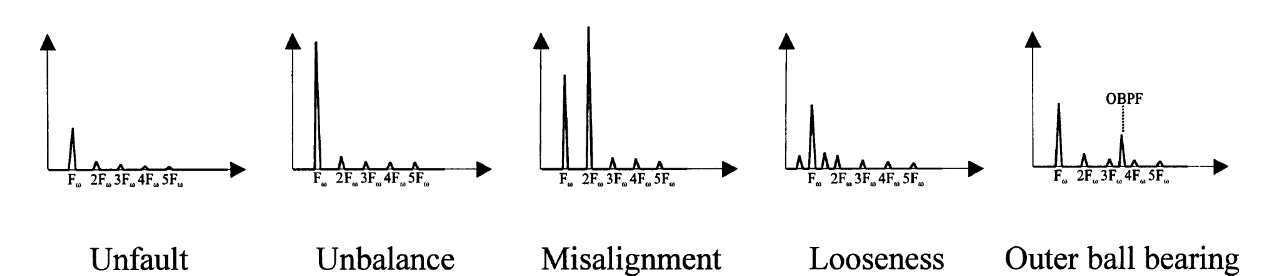
\includegraphics[width=\linewidth]{figures/FaultsAndUnfaults.png}
\caption{Fault and unfault spectrum graphs \cite{Betta2002}.}
\label{fig:faultsunfaults}
\end{figure}

The procedure to calculate critical frequencies involves two steps: first computing the bearing frequency factors, then deriving the vibration frequencies. The following analysis covers the case where the inner race rotates while the outer race remains stationary.

\begin{align}
	F_{\text{OR}} &= \frac{Z}{2} \left(1 - \frac{d}{D} \cos\alpha\right) 
	&&\text{(Outer Race Fault)} \label{eq:OR} \\
	F_{\text{IR}} &= \frac{Z}{2} \left(1 + \frac{d}{D} \cos\alpha\right) 
	&&\text{(Inner Race Fault)} \label{eq:IR} \\
	F_{\text{FTF}} &= \frac{1}{2} \left(1 - \frac{d}{D} \cos\alpha\right) 
	&&\text{(Cage Frequency, Inner Race Rotating)} \label{eq:FT} \\
	F_{\text{BS}} &= \frac{D}{d} \left[1 - \left(\frac{d}{D}\right)^2 \cos^2\alpha\right] 
	&&\text{(Ball Spin Frequency)} \label{eq:BS}
\end{align}

Then, the aforementioned factors when multiplied with shaft speed ($f$) give specific critical bearing vibration frequencies:
\begin{align}
	\text{BPFO} &= f \times F_{\text{OR}} \label{eq:BPFO} \\
	\text{BPFI} &= f \times F_{\text{IR}} \label{eq:BPFI} \\
	\text{BSF}  &= f \times F_{\text{BS}} \label{eq:BSF} \\
	\text{FTF}  &= f \times F_{\text{FTF}} \label{eq:FTF}
\end{align}

where:
\begin{align*}
	&f    &&: \text{Shaft rotational speed (\si{\hertz})} \\
	&\text{BPFI} &&: \text{Ball pass frequency, inner race} \\
	&\text{BPFO} &&: \text{Ball pass frequency, outer race} \\
	&\text{FTF}  &&: \text{Fundamental train frequency} \\
	&\text{BSF}  &&: \text{Ball spin frequency} \\
	&Z    &&: \text{Number of rolling elements} \\
	&D    &&: \text{Pitch circle diameter of the bearing (\si{\milli\meter})} \\
	&d    &&: \text{Rolling element (ball) diameter (\si{\milli\meter})} \\
	&\alpha &&: \text{Contact angle (\si{\degree})} \\
\end{align*}

It is also worth noting that the bearing frequency factors can be obtained through: 
\begin{itemize}
	\item Manufacturer-provided values
	\item Direct calculation using the above equations \eqref{eq:OR}--\eqref{eq:BS}
	\item Reverse calculation from measured vibration frequencies \eqref{eq:BPFO}--\eqref{eq:FTF}
\end{itemize}

To summarize the preceding analysis, Figure \ref{fig:faultTree} provides a clear visualization of the fault diagnosis procedure. When analysis reveals elevated frequency tones, a systematic approach must be followed to identify the source of these dominant frequencies. This process essentially involves mapping characteristic vibration patterns to specific machine faults on a frequency spectrum plot.

\begin{figure}[h]
	\centering
	\begin{tikzpicture}[node distance=1.5cm]
		\node (box1) [draw, rectangle] at (0,0) {Unfault model};
		\node (box2) [draw, rectangle, left of=box1, node distance=6cm] {Fault model};
		\node (box3) [draw, rectangle] at (-7.5,-2) {Unbalance};
		\node (box4) [draw, rectangle] at (-2,-2) {Misalignment};
		\node (box5) [draw, rectangle] at (-5,-2) {Bearing failure};
		\node (box6) [draw, rectangle] at (-10,-2) {Looseness};
		\node (box7) [draw, rectangle] at (-6,-4) {BPFO};
		\node (box8) [draw, rectangle] at (-2,-4) {BPFI};
		\node (box9) [draw, rectangle] at (-4,-4) {BSF};
		\node (box10) [draw, rectangle] at (-8,-4) {FTF};
		
		% Arrows with labels
		\draw[->] (box2) -- node[midway, above] {No} (box1);
		\draw[->] (box2) -- (box3);
		\draw[->] (box2) -- (box4);
		\draw[->] (box2) -- (box5);
		\draw[->] (box2) -- (box6);
		\draw[->] (box5) -- (box7);
		\draw[->] (box5) -- (box8);
		\draw[->] (box5) -- (box9);
		\draw[->] (box5) -- (box10);
	\end{tikzpicture}
	\caption{Fault tree analysis diagram showing the relationship between machine conditions and specific fault frequencies.} \label{fig:faultTree}
\end{figure}

It must be that a fault-emulation method can be used in such cases to simulate the faulty models. This entails that additional tones can be stressed, and crucial spectra modifications may take place for research and comparison purposes.
}


}




\section{Algorithms and Technologies}
% Summary of FFT, data flow, etc.
\subsection{Signal Processing}
\subsubsection{Fast Fourier Transform (FFT)}
{
The Fast Fourier Transform (FFT) is an efficient algorithm for computing the Discrete Fourier Transform (DFT) and its inverse. One of the most prominent FFT algorithms, the Cooley-Tukey algorithm \cite{CooleyTukey1965}, employs a divide-and-conquer approach to reduce the computational complexity from $\mathcal{O}(n^2)$ (for the naive DFT) to $\mathcal{O}(n \log n)$, enabling significant speedups for large amount of data. The mathematical formulation, given a waveform $x_0, x_1, \dots, x_{n-1}$, containing real values, is structured as follows:
\begin{equation}
	X(j) = \sum_{k=0}^{n-1} x(k) \exp\left( - \frac{i2\pi jk}{n} \right) \quad, \text{for} \quad j = 0,1,\dots,n-1
	\label{eq:FFT}
\end{equation}

This reduces complexity from $\mathcal{O}(n^2)$ (naive DFT) to $\mathcal{O}(n \log n)$ (see \eqref{eq:FFT}), enabling major time savings for complex and large-scale transforms. It is also worth articulating that the complexity can be interpreted as the number of operations executed \cite{CooleyTukey1965}, \cite{Singeleton1967}. 

This algorithm is implemented in major numerical packages including MATLAB and NumPy's FFT routines \cite{FFT}. What is highlighted  by Singeleton is that the Cooley-Tukey approach is considerably faster and decently performing especially when coupled with some additional practices so as to execute the Fast Fourier Transform \cite{Singeleton1967}. 

The computation time according to the aforementioned article decreases drastically by making use of the Cooley-Tukey algorithm. In addition, this very algorithm performs and adapts better to different applications compared to Good's, Danielson's and Goertzel's approaches.

It is hereby worth it elaboration on the Fast Fourier Transform algorithm \cite{CooleyTukey1965}.
}

\subsection{Embedded Systems \& IoT}
\subsubsection{ADXL335 Sensor}
Analog signal from sensor breakout to arduino. To elaborate on signal transferring
\begin{itemize}
\item what a sensor breakout is
\item what analog signal is
\end{itemize}


\subsubsection{Arduino Microcontroller}
UART serial communication sending data to RPi. To elaborate on this protocol
\begin{itemize}
\item what serial protocol is
\item what Arduino is
\end{itemize}

\subsubsection{Raspberry Pi 4}
RPi receiving data using a script and posing HTTP Post data to a supabase api. Elaborate on this

\begin{itemize}
\item how to collect data and analyse
\item what Raspberry Pi 4 is
\end{itemize}




\subsection{Backend \& Database}
\subsubsection{Supabase}
\begin{itemize}  
	\item PostgreSQL. 
	\item APIs
	\item what http post is
\end{itemize}  

\subsubsection{Vercel and Next.js}
\begin{itemize}  
	\item nextjs 
	\item vercel
\end{itemize} 
    \chapter{System Engineering and Design}  
\label{chap3}  

% ====== Section 1: Requirements ======  
\section{System Requirements} 
{ 
The system is designed for low-cost, real-time vibration monitoring of rotating machinery. This set-up encompasses components that are of major importance and its aim is to collect data within a specific - prerequired range, store data safely at a database and finally process data.

The following sections include more detailed overview of the system requirements. Hereunder, more details will be elaborated.
}

\subsection{Functional Requirements} 
{ 
The most commonly rotating speed of machinery goes up to 1500 [rpm] corresponds to 25 [Hz]. This relationship is defined by the following equation: 

\begin{equation}
	f \, [\mathrm{Hz}] = \frac{r \, [\mathrm{RPM}]}{60}
\end{equation}

All in all, the functional requirements:

\begin{itemize}  
	\item \textbf{Frequency Range}: 0–300 Hz (covers common machine faults like imbalance, misalignment).  
	\item \textbf{Real-Time Processing}: On-the-fly FFT computation for immediate fault detection.  
	\item \textbf{Scalability}: Modular design for multi-sensor deployments.  
\end{itemize}  
}

\subsection{Non-Functional Requirements} 
{ 
\begin{itemize}  
	\item \textbf{Cost}: Minimize BOM cost (justifies Arduino + RPi4 over industrial PLCs).  
	\item \textbf{Power}: Optimize for continuous operation (e.g., no active cooling).  
	\item \textbf{Accuracy}: ADXL335’s ±3g range suffices for industrial vibrations (cite datasheet).  
\end{itemize}  
}

% ====== Section 2: Hardware Design ======  
\section{Hardware Architecture}  
\subsection{Component Selection}  
{
\begin{itemize}  
	\item \textbf{ADXL335 Accelerometer}:  
	\begin{itemize}  
		\item Analog output simplifies Arduino ADC interfacing.  
		\item 300Hz bandwidth meets requirements (vs. digital sensors like MPU6050 needing I2C).  
	\end{itemize}  
	\item \textbf{Arduino Uno}:  
	\begin{itemize}  
		\item Handles analog sampling at 600Hz (Nyquist-compliant for 300Hz signals).  
		\item Low-latency preprocessing (e.g., DC removal, windowing).  
	\end{itemize}  
	\item \textbf{Raspberry Pi 4}:  
	\begin{itemize}  
		\item Runs Python-based FFT (e.g., NumPy) and SQLite for local storage.  
		\item WiFi/Bluetooth enables cloud integration (e.g., AWS IoT, InfluxDB).  
	\end{itemize}  
\end{itemize}  

\begin{figure}[h]  
	\centering  
	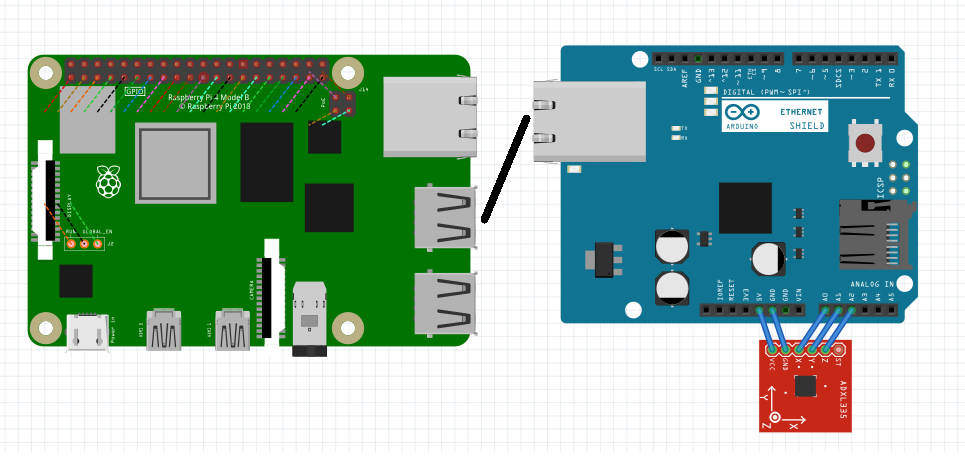
\includegraphics[width=\linewidth]{figures/System.png}  
	\caption{Hardware architecture with signal flow}  
	\label{fig:System}  
\end{figure}
}  

% ====== Section 3: Software & Data Flow ======  
\section{Software Architecture and Data Flow}
 
\subsection{Signal Processing Pipeline} 
{
The Arduino samples data at 600Hz, which is extremely high and constitutes a sufficient sample rate for this project. Additionally, another consideration is receiving data from the ADXL335 sensor breakout, which could potentially make this procedure slower. The highest data volume over a predefined time span achieved for this project is 300Hz.

In essence, a batch of data is received through this procedure by a Raspberry Pi 4, which in turn processes and analyzes these samples.
}  

\subsection{Scalability Considerations}
{  
\begin{itemize}  
	\item \textbf{Multi-Threading}: RPi4 handles concurrent sensor inputs (e.g., 4x Arduino nodes).  
	\item \textbf{Data Compression}: FFT bin reduction (0–300Hz only) minimizes cloud costs.  
\end{itemize}  

\begin{figure}[h]  
	\centering  
	\begin{tikzpicture}[node distance=1.5cm]  
		\node (sensor) [draw, rectangle] {ADXL335};  
		\node (arduino) [draw, rectangle, below of=sensor] {Arduino};  
		\node (rpi) [draw, rectangle, below of=arduino] {Raspberry Pi 4};  
		\node (cloud) [draw, rectangle, below of=rpi] {Cloud DB};  
		
		\draw[->] (sensor) -- node[right] {Analog (0–300Hz)} (arduino);  
		\draw[->] (arduino) -- node[right] {UART (600SPS)} (rpi);  
		\draw[->] (rpi) -- node[right] {WiFi/HTTP} (cloud);  
	\end{tikzpicture}  
	\caption{End-to-end data flow with protocols}  
	\label{fig:Flowchart}  
\end{figure}  
}

\subsection{Arduino sketch}
{
Elaboration on (including the whole code):
\begin{itemize}
\item Description of sketch and cpp files
\item elaborate on how it shares data via UART
\item Analyse the possibility of translating Voltage into g or m/s2
\end{itemize}
}

\subsection{Raspberry Pi coding}
{
Elaboration on (including some parts of the code):
\begin{itemize}
\item Description of the whole program
\item how it posts data via HTTP
\item Data stored on database , and database setup
\end{itemize}
}

\subsection{Vercel coding}
{
Elaboration on (including some parts of the code):
\begin{itemize}
\item page file that prints data
\item how it is coupled with supabase
\end{itemize}
}

    \chapter{Results}
\label{chap4}

\section{Intro}
Results

\section{A}

\subsection{Τίτλος Υπο-ενότητας}

\subsection{Τίτλος Υπο-ενότητας}

\subsection{Τίτλος Υπο-ενότητας}

etc.

    \chapter{Conclusions}
\label{chap_last}
Εδώ εξηγούμε ότι θα συνοψίσουμε την μελέτη που εκπονήθηκε στα πλαίσια της διπλωματικής.
{
\begin{itemize}
\item summarize how it decides if a bearing is defective
\item how it collects data
\item how data is analysed and at what stages it is analysed
\end{itemize}
}

\section{Σύνοψη και συμπεράσματα}
Εδώ συνοψίζουμε τα αποτελέσματα της διπλωματικής και περιγράφουμε τα συμπεράσματα που προέκυψαν, αρνητικά και θετικά. Επιβεβαιώνουμε την συνεισφορά της διπλωματικής στα προβλήματα που αναφέραμε στην εισαγωγή.
{

}

\section{Μελλοντικές επεκτάσεις}
Εδώ δίνουμε ιδέες για επέκταση της διπλωματικής.
{

}

%
%%%%%%%%%%%%%%%%%%%%%%%%%%%%%%%%%%%%%%%%%%%%%%%%%%%%


%\backmatter % μην ενεργοποιείτε την εντολή
% Βιβλιογραφία - Αναφορές
	\bibliography{bibliography/references}


%%%%%%%%%%%%%%%%%%%%%%%%%%%%%%%%%%%%%%%%%%%%%%%%%%%%%
%% APPENDICES (optional) / ΠΑΡΑΡΤΗΜΑΤΑ (ΠΡΟΑΙΡΕΤΙΚΑ)
%%

    % Να μην τροποποποιηθεί

\cleardoublepage\thispagestyle{plain}
~\vfill
\ifgrthesisoption
    \centerline{\huge\bf ΠΑΡΑΡΤΗΜΑΤΑ}\phantomsection
    \addcontentsline{toc}{chapter}{ΠΑΡΑΡΤΗΜΑΤΑ}
\else
    \centerline{\huge\bf APPENDICES}\phantomsection
    \addcontentsline{toc}{chapter}{APPENDICES}
\fi
\vfill

% Μην τροποποιήσετε τις ακόλουθες εντολές
\ifgrthesisoption
    \renewcommand{\chaptername}{Παράρτημα}
\else
    \renewcommand{\chaptername}{Appendix}
\fi

   \renewcommand{\thechapter}{} 
   \renewcommand{\thesection}{\arabic{section}}

   % Μεμονωμένο Παράρτημα 
% ορίζεται ο τίτλος του παραρτήματος
\edef\chaptertitle{Τίτλος Παραρτήματος}
\label{appendix}

% Μην τροποποιήσετε τις ακόλουθες εντολές
\chapter*{\chaptername\\\vspace{1cm} \chaptertitle} 
\addcontentsline{toc}{chapter}{\chaptername\texorpdfstring{\\}~\chaptertitle}
\setcounter{section}{0}
\renewcommand{\chaptermark}[1]{\markboth{\textit{\chaptername. \chaptertitle}}{}}
\chaptermark{}


Τα παραρτήματα περιλαμβάνουν συνοδευτικό, υποστηρικτικό υλικό (πίνακες, φωτογραφίες, ερωτηματολόγια, στατιστικά στοιχεία, αποδείξεις, περιγραφές  λογισμικών  προγραμμάτων,  παραδείγματα,  περιγραφές 
πολύπλοκων διαδικασιών, λίστα με πρωτογενή στοιχεία, λεπτομερής περιγραφή και προδιαγραφές εξοπλισμού, οδηγίες εγκατάστασης λογισμικού, κ.λπ.), ή αλλιώς ό,τι θεωρείται χρήσιμο να περιγραφεί, αλλά δεν συνηθίζεται να 
εντάσσεται μέσα στο κυρίως κείμενο της Εργασίας.  Στο κυρίως κείμενο της Εργασίας πρέπει να γίνονται οι κατάλληλες παραπομπές προς τα παραρτήματα, όπου το κείμενο σχετίζεται με υλικό που περιλαμβάνεται σε αυτά. Ένα παράρτημα, αναλόγως με το περιεχόμενό του, μπορεί να είναι ενιαίο, ή να χωρίζεται σε ενότητες.


\section{Δυνατότητες του \LaTeX}

Kαθώς το παρόν αποτελεί ένα πρότυπο συγγραφής διπλωματικών εργασιών, στην ενότητα αυτή επιδεικνύονται ορισμένες από τις δυνατότητες το \LaTeX οι οποίες μπορούν να αξιοποιηθούν στο κείμενο μιας διπλωματικής εργασίας (μια καλή πηγή για τη διερεύνηση των δυνατοτήτων του \LaTeX είναι η ιστοσελίδα {\small\url{https://www.overleaf.com/learn/latex/Main_Page}}).

\subsection{Πίνακες}
Ο Πίνακας~\ref{tab1} είναι ένα παράδειγμα πίνακα σχεδιασμένου με εντολές του περιβάλλοντος \texttt{tabular}.
\begin{table}[htb]
\centering
\caption{Παράμετροι πειραμάτων}
\label{tab1}
\begin{tabular}{|c|>{\centering\arraybackslash}m{8cm}|}
\hline Πλήθος κελιών καννάβου \textit{{c}} $\times$ \textit{{c}} & 50 $\times$ 50, 100 $\times$ 100, 200 $\times$ 200, \textbf{250} $\times$ \textbf{250}, 500 $\times$ 500, 1000 $\times$ 1000  \\
\hline Τυπική απόκλιση $\sigma$ & 25{m}, 50{m}, 75{m}, \textbf{100{m}}, 150{m}, 200{m} \\
\hline Αριθμός εγγύτερων γειτόνων \textit{{k}} & 1, 2, \textbf{3}, 4, 5, 10, 20 \\
\hline Πιθανοτικό κατώφλι $\theta$ & 50$\%$, 60$\%$, 70$\%$, \textbf{75$\%$}, 80$\%$, 90$\%$, 99$\%$ \\
\hline  
\end{tabular}

\end{table}

\subsection{Διαγράμματα - Γραφικές παραστάσεις}
Στο Σχήμα~\ref{fig1}, παρουσιάζεται ένα παράδειγμα γραφικής παράστασης σχεδιασμένης με το Gnuplot.
\begin{figure}[htb]
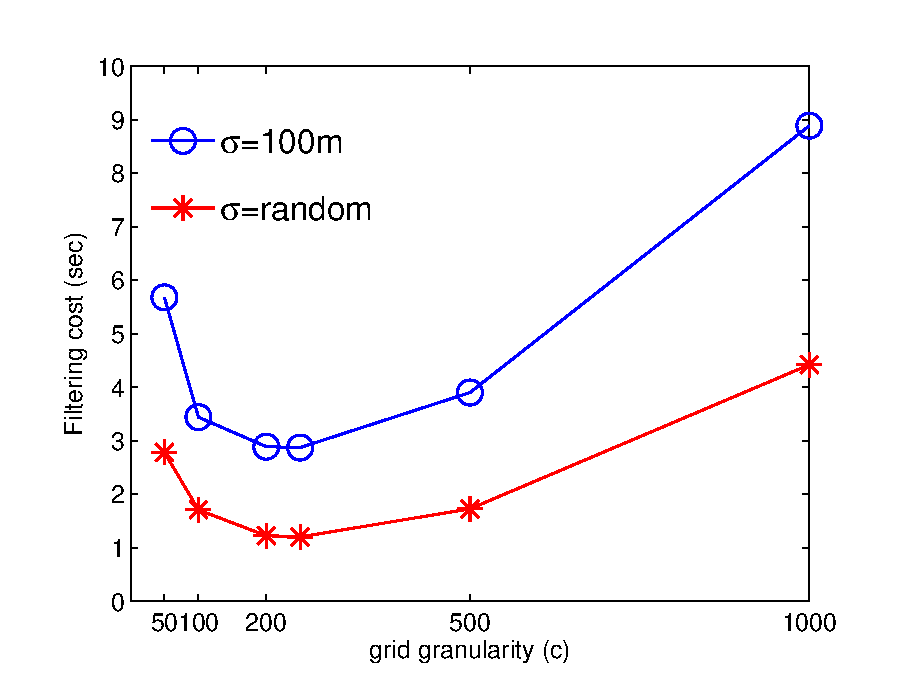
\includegraphics[scale=0.7]{figures/grid_granularity.eps}
\centering
\caption{Κλιμάκωση χρόνου εκτέλεσης για διάφορες υποδιαιρέσεις του καννάβου}	
\label{fig1}
\end{figure} 

\subsection{Σχήματα}
Ακολουθεί στο Σχήμα~\ref{fig2} ένα παράδειγμα σχήματος φτιαγμένου με εντολές του πακέτου Ti\textit{k}Z.
\begin{figure}[htb]
\begin{center}
\begin{tikzpicture}
\draw (-2,0) -- (2,0);
\filldraw [gray] (0,0) circle (2pt);
\draw (-2,-2) .. controls (0,0) .. (2,-2);
%\draw (-2,2) .. controls (-1,0) and (1,0) .. (2,2);
 \draw[gray, thick] (-1,2) -- (2,-4);
\draw[gray, thick] (-1,-1) -- (2,2);
\filldraw[black] (0,0) circle (2pt)  ;
\end{tikzpicture}
\end{center}
\caption{Παράδειγμα σχήματος με εντολές του πακέτου Ti\textit{k}Z}	
\label{fig2}
\end{figure}

\subsection{Αλγόριθμοι}
Ακολουθεί ο Αλγόριθμος~\ref{alg1}, ο οποίος είναι μορφοποιημένος με τα πακέτα algorithm και algorithmic.

\begin{algorithm}[htb]
\caption{\ \ \ Probabilistic $k\theta NN$ Monitoring}
\begin{algorithmic}[1]
\begin{small}

\STATE{\bf Procedure} {\em VerifyCandidate} (focal query point $q$, threshold $\theta$, object $o$, list of auxiliary objects $P$, distance $kMAXDIST$) 

\IF { $\Phi(o, kMAXDIST) \geq \theta$ {\bf and} $L_2(q, o) \leq L_2(q, P.$top()) }

\STATE {$P$.pop()};   \ \ \ \ \ \ \ \ {\em //Replace the most extreme element in $P$, since candidate $o$ ... }

\STATE {$P$.push($o$)};  \ \ \ \ \ {\em //... has enough probability and has its mean closer to focal $q$ }

\ENDIF

\STATE {\bf End Procedure}


\end{small}
\end{algorithmic}
\label{alg1}
\end{algorithm}

\subsection{Μαθηματικές εκφράσεις}
Ακολουθούν παραδείγματα μαθηματικών εκφράσεων.
\begin{eqnarray}
\hat{I}(x,u,t)     &=& dist(y(t_f),\Gamma)
+  \int_t^{t_f} \: {\cal L}( y(s),u(s),s) \: ds
\label{con11b}
\end{eqnarray}

     \[
        \frac{d}{dx}\left( \int_{0}^{z} f(u)\,du\right)=f(x).
     \]

\subsection{Θεωρήματα, Πορίσματα, Ορισμοί, κλπ.}

Ακολουθεί παράδειγμα θεωρήματος από την ιστοσελίδα  {\small\url{https://www.overleaf.com/learn/latex/Theorems_and_proofs}}

\begin{theorem}
Let $f$ be a function whose derivative exists in every point, then $f$ 
is a continuous function.
\end{theorem}

\subsection{Απαριθμήσεις}

Μια απαρίθμηση (itemized list) βοηθά στην παρουσίαση μιας σειράς περιπτώσεων με σαφήνεια.
Ακολουθεί παράδειγμα.

H εκπαίδευση στην Ελλάδα διακρίνεται σε:
\begin{itemize}
\item Πρωτοβάθμια 
\item Δευτεροβάθμια 
\item Τριτοβάθμια 
\end{itemize}

\subsection{Είδη πηγών στις αναφορές}

Στο references.bib μπορεί να δει κανείς πώς γράφονται διάφορα είδη πηγών 
(Βιβλία Ξενόγλωσσα \cite{goossens93},
Βιβλία Ελληνικά \cite{greekbook},
Άρθρα σε επιστημονικά περιοδικά \cite{LiArTs13},
Άρθρα σε επιστημονικά συνέδρια \cite{dcis2011},
Ιστοσελίδες \cite{LaTeXProject},
Πτυχιακές Εργασίες \cite{elli05},
Διπλωματικές Εργασίες \cite{zoi04},
Μεταπτυχιακές Διπλωματικές Εργασίες \cite{master04},
Διδακτορικές Διατριβές \cite{phd045},
Τεχνικές Αναφορές \cite{MSU-CSE-05-29},
Διπλώματα Ευρεσιτεχνίας \cite{viswanathan2014convenient}),
Κεφάλαια σε συλλογικούς τόμους
\cite{[PS11]}.

 

%
%%%%%%%%%%%%%%%%%%%%%%%%%%%%%%%%%%%%%%%%%%%%%%%%%%%%


\end{document}